\chapter{Siêu không gian và việc xây dựng động lực học siêu đối xứng}

\lectureoverview{Chúng ta xây dựng lại siêu đối xứng từ hệ nhỏ nhất mà nó có thể tác dụng lên: một dao động tử boson và một dao động tử fermion có cùng năng lượng. Sự tương phản giữa các phương trình bậc hai và bậc nhất của chúng dẫn đến các siêu điện tích và đại số của chúng. Sau đó ta diễn giải lại đại số ấy như hình học trên một không gian với tọa độ thông thường (t) và các tọa độ Grassmann \(\theta,\bar\theta\). Các siêu trường gộp boson, fermion và một trường phụ trợ vào một đối tượng duy nhất; phép tích phân Berezin rút ra một Lagrangian thông thường bất biến; các đạo hàm hiệp biến làm cho các ràng buộc tương thích với đối xứng trở nên khả dĩ; và ràng buộc chiral cung cấp ví dụ quan trọng đầu tiên. Bài giảng cố ý phơi bày các khó khăn về dấu và thứ tự của bộ máy này, rồi kết thúc bằng việc giải thích vì sao bản thân đối xứng còn cơ bản hơn một danh mục các quy tắc Feynman.}

\section{Trở lại hệ một mode}

Hãy bắt đầu lại với fermion và boson ở trạng thái nghỉ. Ta lược bỏ mọi tọa độ không gian và mọi nhãn động lượng. Trong một mode cho trước, một lượng tử có mặt hoặc vắng mặt, và các toán tử tạo, hủy là đủ để mô tả nó. Viết \(a^\dagger,a\) cho một mode boson và \(c^\dagger,c\) cho một mode fermion. Chúng thỏa mãn
\begin{align}
[a,a^\dagger]&=1,
&
\{c,c^\dagger\}&=1,
&
c^2=(c^\dagger)^2&=0.
\end{align}
Nếu hai lượng tử có cùng năng lượng \(m\), thì, ngoài một hằng số chân không không quan trọng,
\begin{equation}
H=m\left(a^\dagger a+c^\dagger c\right).
\label{eq:l7-one-mode-hamiltonian}
\end{equation}
Toán tử số \(a^\dagger a\) có thể nhận mọi giá trị nguyên không âm, còn \(c^\dagger c\) chỉ có thể bằng 0 hoặc 1. Đó là toàn bộ động học của mô hình đồ chơi này.

Sự đơn giản hóa này mang tính chiến lược. Ta muốn hiểu phép toán hủy một boson và tạo một fermion, hoặc làm điều ngược lại, mà không làm thay đổi năng lượng. Tuy nhiên, trước khi xây dựng phép toán đó, ta sẽ chuyển cùng hệ ấy từ ngôn ngữ toán tử sang ngôn ngữ Lagrangian.

\section{Dao động tử boson}

Đối với boson, đưa vào một tọa độ thực \(\phi(t)\). Khi không có biến thiên theo không gian, một trường vô hướng tự do trở thành một dao động tử điều hòa thông thường. Biểu thức đầu tiên được viết trên bảng là
\[
\frac{1}{2}\dot\phi^{,2}+\frac{1}{2}m^2\phi^2.
\]
Biểu thức đó là động năng cộng thế năng, không phải Lagrangian. Dấu được sửa ngay trong bài giảng:
\begin{equation}
L_B=\frac{1}{2}\dot\phi^{,2}-\frac{1}{2}m^2\phi^2.
\label{eq:l7-boson-lagrangian}
\end{equation}

\begin{figure}[H]
\centering
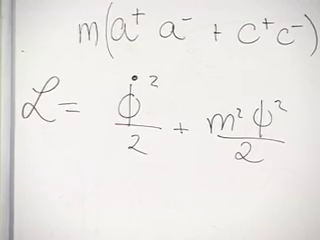
\includegraphics[width=0.62\textwidth]{lecture_07_figure_02.png}
\lectureframe{00:03:25.431}
\caption{Hamiltonian một mode ở phía trên Lagrangian boson. Khung hình giữ lại dấu cộng ban đầu trước khi được sửa bằng lời thành \(T-V\).}
\end{figure}

\begin{classroomqa}
\audiencequestion{Dấu trong Lagrangian dao động tử đang hiển thị sai ở chỗ nào? \lecturetimestamp{00:04:00}}
\lecturerresponse{Năng lượng là \(T+V\), còn Lagrangian là \(T-V\). Vì vậy số hạng thế phải mang dấu trừ. Sự hiệu chỉnh này biến phương trình từ hành vi mũ thành dao động điều hòa như dự định.}
\end{classroomqa}

Thật vậy, phương trình Euler--Lagrange cho
\begin{align}
\frac{d}{dt}\frac{\partial L_B}{\partial\dot\phi}
&=\frac{\partial L_B}{\partial\phi},\\
\ddot\phi&=-m^2\phi,
\end{align}
hoặc
\begin{equation}
\ddot\phi+m^2\phi=0.
\label{eq:l7-boson-eom}
\end{equation}
Tần số của nó là \(m\), không phải \(m^2\). Lượng tử hóa dao động tử này tạo ra cùng một thang trạng thái được mô tả bởi \(a^\dagger\) và \(a\) trong phương trình~\eqref{eq:l7-one-mode-hamiltonian}.

\section{Vì sao tác dụng của fermion là bậc nhất}

Lagrangian fermion trông đơn giản hơn vì nó chỉ chứa một đạo hàm theo thời gian. Lý do đã lộ ra ngay trong một phép thử cố ý ngây thơ. Với một biến giao hoán thông thường,
\begin{equation}
L_{\mathrm{trial}}=\phi\dot\phi
=\frac{1}{2}\frac{d}{dt}\phi^2.
\end{equation}
Đó là một đạo hàm toàn phần. Phương trình Euler--Lagrange của nó chỉ nói \(\dot\phi=\dot\phi\), nên mọi quỹ đạo khả vi đều được phép. Loại bỏ một đạo hàm toàn phần khỏi tác dụng làm thay đổi dữ liệu ở biên chứ không làm thay đổi phương trình chuyển động trong nội miền.

Bây giờ hãy đổi tên biến thành \(\psi\) và tuyên bố nó là lẻ Grassmann. Cả \(\psi\) lẫn \(\dot\psi\) đều phản giao hoán. Với lựa chọn cố định là biến phân bên trái, việc sắp xếp lại các thừa số lẻ đưa vào một dấu trừ, nên cùng phép thử hình thức đó cho
\begin{equation}
\frac{d}{dt}\frac{\partial L_{\mathrm{trial}}}{\partial\dot\psi}
=\dot\psi,
\qquad
\frac{\partial L_{\mathrm{trial}}}{\partial\psi}
=-\dot\psi.
\end{equation}
Vì vậy phương trình là
\begin{equation}
\dot\psi=-\dot\psi
\quad\Longrightarrow\quad
\dot\psi=0.
\label{eq:l7-constant-fermion}
\end{equation}
Biểu thức vốn là một hằng đẳng thức đối với một tọa độ giao hoán nay đã có nội dung động lực học đối với một tọa độ phản giao hoán. Nó có quá nhiều nội dung đối với một dao động tử, vì nó chỉ cho phép một hằng số, nhưng chính đó lại là đầu mối ta cần.

\begin{classroomqa}
\audiencequestion{Có phải nghiệm đơn giản chỉ là \(\psi\) là hằng số không? \lecturetimestamp{00:13:57}}
\lecturerresponse{Đúng. Phương trình~\eqref{eq:l7-constant-fermion} là một phương trình vi phân bậc nhất đích thực, và nghiệm của nó là một hằng tùy ý nhận giá trị Grassmann. Một số hạng khối lượng sẽ biến nghiệm tĩnh ấy thành một nghiệm dao động.}
\end{classroomqa}

Cố gắng hiển nhiên, \(m\psi^2\), thất bại vì \(\psi^2=0\). Ta cần hai biến lẻ thực \(\psi_1,\psi_2\), hoặc tương đương là một biến phức và liên hợp của nó. Bài giảng triển khai dạng hai biến thực trên bảng, liên tục kiểm tra các dấu và các hệ số 2. Một dạng phức được chuẩn hóa theo quy ước là
\begin{equation}
L_F=\frac{i}{2}
\left(\bar\psi\dot\psi-\dot{\bar\psi}\psi\right)
-m\bar\psi\psi.
\label{eq:l7-fermion-lagrangian}
\end{equation}
Sai khác bởi một đạo hàm toàn phần, biểu thức này là \(i\bar\psi\dot\psi-m\bar\psi\psi\). Biến phân theo \(\bar\psi\) cho
\begin{equation}
i\dot\psi=m\psi,
\qquad
\psi(t)=\psi(0)e^{-imt}.
\label{eq:l7-fermion-eom}
\end{equation}
Phương trình liên hợp có pha ngược lại. Vì thế mode fermion dao động với năng lượng \(m\), cũng như mode boson, mặc dù phương trình của nó là bậc nhất chứ không phải bậc hai.

\editorialnote{Phương trình~\eqref{eq:l7-fermion-lagrangian} cố định một quy ước chuẩn về thứ tự và chuẩn hóa cho phép tính thăm dò với hai biến thực. Chính bài giảng đưa vào thừa số \(i\), điều chỉnh một hệ số 2, và để ngỏ một dấu của một thành phần thực. Những thay đổi này không làm thay đổi kết luận trung tâm của nó: động học fermion là bậc nhất, khối lượng xuất hiện tuyến tính, và một fermion phức cho một song tuyến tính khác không.}

Đây là hình chiếu không chiều của một sự tương phản tương đối tính quen thuộc. Phương trình Klein--Gordon là bậc hai theo thời gian, còn phương trình Dirac là bậc nhất. Khi đã lược bỏ không gian, boson là một dao động tử điều hòa và fermion là một dao động tử Grassmann phức.

\begin{classroomqa}
\audiencequestion{Thứ tự viết \(\psi\), \(\dot\psi\) và các liên hợp của chúng có quan trọng không? \lecturetimestamp{00:18:58}}
\lecturerresponse{Các công thức trung gian quả thật phụ thuộc vào thứ tự vì các thừa số lẻ phản giao hoán. Lý thuyết vật lý thì không phụ thuộc vào một sở thích ghi chép tùy tiện, miễn là từ đầu đến cuối người ta dùng một quy ước duy nhất cho biến phân trái hay phải, phép liên hợp và phép tích phân. Đảo thứ tự một cặp lẻ làm đổi một dấu, và dấu ấy phải được đổi một cách nhất quán ở mọi chỗ khác.}
\end{classroomqa}

Kết hợp các phương trình~\eqref{eq:l7-boson-lagrangian} và \eqref{eq:l7-fermion-lagrangian} cho một mô tả Lagrangian của cùng một cặp tương ứng đã được biểu diễn bởi phương trình~\eqref{eq:l7-one-mode-hamiltonian}. Giờ đây ta đã sẵn sàng nhận diện đối xứng giữa chúng.

\section{Siêu điện tích và đại số của chúng}

Một toán tử hủy một fermion và tạo một boson là
\begin{equation}
Q^\dagger=\sqrt{2m}\,a^\dagger c,
\end{equation}
trong khi liên hợp của nó hủy một boson và tạo một fermion,
\begin{equation}
Q=\sqrt{2m}\,a c^\dagger.
\end{equation}
Sự chuẩn hóa được chọn sao cho đại số có dạng chuẩn. Dùng \(cc^\dagger=1-c^\dagger c\), \(aa^\dagger=a^\dagger a+1\), và thực tế rằng các toán tử boson và fermion giao hoán với nhau,
\begin{align}
\{Q,Q^\dagger\}
&=2m\left(ac^\dagger a^\dagger c+a^\dagger c a c^\dagger\right)\notag\\
&=2m\left[(a^\dagger a+1)c^\dagger c
+a^\dagger a(1-c^\dagger c)\right]\notag\\
&=2m\left(a^\dagger a+c^\dagger c\right)=2H.
\label{eq:l7-superalgebra}
\end{align}
Các toán tử boson có thể được chuyển qua các toán tử fermion. Chính tính lũy linh vốn giới hạn số chiếm chỗ fermion cho
\begin{equation}
Q^2=(Q^\dagger)^2=0.
\end{equation}
Cuối cùng,
\begin{equation}
[H,Q]=[H,Q^\dagger]=0.
\label{eq:l7-conserved-supercharges}
\end{equation}
Mỗi siêu điện tích làm thay đổi số boson và số fermion theo hai chiều ngược nhau, nên hai độ thay đổi năng lượng triệt tiêu nhau khi các tần số bằng nhau.

\begin{classroomqa}
\audiencequestion{\([H,Q]\) là gì? Có phải đáp án tỉ lệ với \(Q\) không? \lecturetimestamp{00:25:10}}
\lecturerresponse{Không. Đáp án bằng 0. Một toán tử tạo hoặc hủy đơn lẻ sẽ nhận năng lượng của nó khi lấy giao hoán với \(H\), nhưng các đóng góp boson và fermion trong \(Q\) triệt tiêu nhau. Sự triệt tiêu ấy chính là điều kiện cùng năng lượng.}
\end{classroomqa}

\begin{classroomqa}
\audiencequestion{Giao hoán tử ấy chẳng phải đã được viết trên bảng rồi sao? \lecturetimestamp{00:25:45}}
\lecturerresponse{Đúng vậy. Việc tìm lại nó vẫn hữu ích vì nó buộc ta phải diễn giải chứ không chỉ chép lại hệ thức: giao hoán với Hamiltonian có nghĩa là phép biến đổi ấy là một đối xứng và bộ sinh của nó được bảo toàn.}
\end{classroomqa}

Tính từ \emph{điện tích} phản ánh định luật bảo toàn này. Tuy nhiên, ta không nên coi \(Q\) như một con số thông thường có thể đo đồng thời gắn với một trạng thái. Nó là lẻ Grassmann, lũy linh, và ánh xạ một trạng thái boson thành một trạng thái fermion. Phát biểu hữu ích là nó là một bộ sinh được bảo toàn, tác động trong các siêu đa bội suy biến.
\editorialnote{Cách diễn đạt này chỉnh lý phép so sánh trên lớp học giữa việc gắn nhãn các trạng thái bằng năng lượng hay điện tích điện. Các siêu điện tích lẻ riêng lẻ, không Hermite, không phải là những quan sát lượng thông thường với các nhãn lượng tử bằng số. Tác động được bảo toàn của chúng và biểu diễn của toàn bộ siêu đại số mới đem lại sự phân loại đúng.}

\section{Các bộ sinh dưới dạng đạo hàm}

Đại số thì súc tích, nhưng tự nó không cho ta biết phải xây dựng các lý thuyết có tương tác như thế nào. Bước tiếp theo mang tính hình học. Những bộ sinh đối xứng quen thuộc vốn đã tác dụng như các toán tử vi phân. Theo quy ước của bài giảng,
\begin{equation}
H=i\frac{\partial}{\partial t},
\qquad
P=-i\frac{\partial}{\partial x}.
\end{equation}

\begin{figure}[H]
\centering
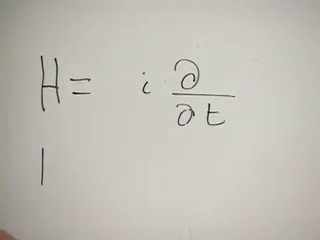
\includegraphics[width=0.50\textwidth]{lecture_07_figure_03.png}
\lectureframe{00:28:12.720}
\caption{Hamiltonian được biểu diễn như bộ sinh của các phép tịnh tiến theo thời gian.}
\end{figure}

Mômen góc cũng tương tự: một tọa độ nhân với một đạo hàm. Nếu các siêu điện tích là các bộ sinh lẻ, thì tự nhiên ta sẽ hỏi liệu chúng có thể được biểu diễn bằng các đạo hàm theo các tọa độ lẻ hay không. Vì vậy ta mở rộng trục thời gian thành siêu không gian
\begin{equation}
(t,\theta,\bar\theta),
\qquad
\theta^2=\bar\theta^2=0,
\qquad
\theta\bar\theta=-\bar\theta\theta.
\end{equation}
Các trường trên không gian này phụ thuộc vào một thời gian thông thường và một cặp tọa độ Grassmann liên hợp.

Bài giảng cố ý cho thấy các dấu dễ gây nhầm lẫn đến mức nào. Dấu do liên hợp phức, dấu do chuyển một tham số lẻ, và dấu do chọn đạo hàm trái thay cho đạo hàm phải tương ứng với những thao tác khác nhau. Thay vì giữ lại các bước trình bày trên bảng vốn không tương thích lẫn nhau, giờ đây ta cố định một quy ước: mọi đạo hàm lẻ đều là đạo hàm trái, và
\begin{equation}
q=\partial_\theta+i\bar\theta\partial_t,
\qquad
\bar q=\partial_{\bar\theta}+i\theta\partial_t.
\label{eq:l7-differential-supercharges}
\end{equation}
Khi đó
\begin{equation}
q^2=\bar q^{,2}=0,
\qquad
\{q,\bar q\}=2i\partial_t=2H.
\label{eq:l7-differential-algebra}
\end{equation}
Hệ số 2 xuất phát từ hai hạng chéo: \(\{\partial_\theta,\theta\}=1\) và \(\{\partial_{\bar\theta},\bar\theta\}=1\). Nếu các toán tử sinh chỉ chứa \(\partial_\theta\) và \(\partial_{\bar\theta}\), thì phản giao hoán tử của chúng sẽ triệt tiêu và không thể tái tạo Hamiltonian.

\begin{classroomqa}
\audiencequestion{Hai số hạng đạo hàm theo thời gian trong \(q\) và \(\bar q\) có phải mang cùng dấu không? \lecturetimestamp{00:31:01}}
\lecturerresponse{Chúng phải được chọn nhất quán sao cho phản giao hoán tử hỗn hợp là \(2H\). Có thể dùng hoặc một quy ước dấu cộng tổng thể, hoặc phương án liên hợp nhất quán của nó. Chính phép tính, chứ không phải trực giác hình ảnh về ký hiệu \(i\), mới quyết định các dấu tương đối.}
\end{classroomqa}

Cả phòng liên tục kiểm tra các dấu, và sự khó khăn trở thành một trò đùa: các dấu dường như thay đổi trên đường đi làm. Trò đùa ấy rất đúng chỗ. Việc phản giao hoán một tham số Grassmann qua một tọa độ có thể làm đổi dấu ngay cả khi không có quy ước vật lý nào thay đổi. Phương trình~\eqref{eq:l7-differential-supercharges} là mốc tham chiếu cố định cho mọi điều tiếp theo.

\subsection{Siêu đối xứng như một phép dịch tọa độ}

Cho \(\xi,\bar\xi\) là các tham số lẻ vô cùng bé. Tác dụng lên một siêu trường bằng
\begin{equation}
\delta_\xi=\xi q+\bar\xi\bar q
\end{equation}
tương đương, theo quy ước ở trên, với phép biến đổi tọa độ vô cùng bé
\begin{align}
\theta&\longrightarrow\theta+\xi,\\
\bar\theta&\longrightarrow\bar\theta+\bar\xi,\\
t&\longrightarrow t+i\left(\xi\bar\theta+\bar\xi\theta\right).
\label{eq:l7-coordinate-shift}
\end{align}
Vì vậy độ biến thiên của một siêu trường vô hướng là
\begin{equation}
\delta_\xi\Phi
=\left(\xi\partial_\theta+\bar\xi\partial_{\bar\theta}
+i\xi\bar\theta\partial_t+i\bar\xi\theta\partial_t\right)\Phi
=\left(\xi q+\bar\xi\bar q\right)\Phi.
\end{equation}
Đây là nội dung hình học của siêu đối xứng. Nó là một phép tịnh tiến theo các hướng lẻ gắn với một phép tịnh tiến theo thời gian thông thường. Hai phép dịch lẻ khép lại thành một phép tịnh tiến theo thời gian do phương trình~\eqref{eq:l7-differential-algebra}.

\begin{classroomqa}
\audiencequestion{Dấu trừ đang bị tranh luận đó có thể biểu diễn một chuyển động lùi về thời gian không? \lecturetimestamp{00:58:13}}
\lecturerresponse{Một quy ước dấu khác có thể đảo chiều phép dịch thời gian vô cùng bé được hiển thị, nhưng không có quá trình vật lý lùi-thời gian riêng biệt nào được đưa vào. Điều quan trọng là phép biến đổi tọa độ và các bộ sinh vi phân tuân theo cùng một đại số.}
\end{classroomqa}

\begin{classroomqa}
\audiencequestion{Thời gian mở rộng này có sự hiện thực hóa vật lý hay chỉ là một công cụ hạch toán hình thức? \lecturetimestamp{00:58:23}}
\lecturerresponse{Theo một nghĩa hữu ích thì đúng là một công cụ hạch toán: nó đóng gói đại số vào hình học. Nhưng sự đóng gói ấy trở nên có giá trị vật lý khi đưa các tương tác vào. Siêu không gian cung cấp một phép tính có hệ thống để xây dựng các Lagrangian bảo toàn đối xứng boson--fermion ở mọi bước, cũng như phép tính tensor giúp ta xây dựng các vô hướng Lorentz.}
\end{classroomqa}

\section{Siêu trường và thành phần phụ trợ}

Vì chỉ có hai tọa độ lẻ, khai triển của một siêu trường chẵn sẽ dừng lại:
\begin{equation}
\Phi(t,\theta,\bar\theta)
=\phi(t)+\bar\theta\psi(t)+\bar\psi(t)\theta
+D(t)\bar\theta\theta.
\label{eq:l7-superfield}
\end{equation}
Hệ số của các đơn thức chẵn, \(\phi\) và \(D\), mang tính boson; hệ số của các đơn thức lẻ, \(\psi\) và \(\bar\psi\), mang tính fermion. Không có hạng \(\theta^2\), \(\bar\theta^2\) hay bậc cao hơn nào còn tồn tại. Ta để phụ thuộc thời gian ở dạng chưa khai triển vì một chuỗi Taylor thông thường theo \(t\) sẽ không dừng lại và ở đây không phục vụ mục đích nào.

\begin{classroomqa}
\audiencequestion{Thành phần \(D(t)\) ở hạng trên cùng là gì? \lecturetimestamp{00:41:46}}
\lecturerresponse{Ở giai đoạn này, nó đơn giản chỉ là hệ số bosonic cuối cùng trong khai triển hữu hạn. Trong tác dụng theo thành phần, nó thông thường không có hạng động năng và bị khử bằng một phương trình chuyển động đại số, nên được gọi là một trường phụ trợ. Bài giảng đùa rằng ``D là viết tắt của dummy,'' điều này nêu bật vai trò không động lực học của nó dù đó không phải là định nghĩa lịch sử.}
\end{classroomqa}

Siêu trường là một đối tượng duy nhất, còn \(\phi,\psi,\bar\psi,D\) là các thành phần của nó. Một phép biến đổi siêu đối xứng trộn lẫn chúng. Vì thế một boson và một fermion có quan hệ với nhau theo gần như cùng nghĩa cấu trúc mà các thành phần \(x\)- và \(y\)- của một vectơ có quan hệ với nhau dưới một phép quay, mặc dù không thể hình dung các phương Grassmann như các trục thông thường.

\section{Siêu tác dụng và thành phần trên cùng}

Để thu được các phương trình chuyển động, ta cần một tác dụng. Trong lý thuyết trường thông thường, người ta lập một Lagrangian vô hướng và tích phân nó trên không-thời gian. Ở đây biểu thức tương tự là
\begin{equation}
S=\int dt\,d\theta\,d\bar\theta\;\Lambda
\bigl(\Phi,\text{ superspace derivatives of }\Phi\bigr),
\label{eq:l7-superaction}
\end{equation}
trong đó \(\Lambda\) là một siêu trường chẵn. Tích phân Berezin là đại số. Ta chọn
\begin{equation}
\int d\theta\,d\bar\theta\;\bar\theta\theta=1.
\end{equation}
Vì vậy, nếu
\begin{equation}
\Lambda=A+\bar\theta B+\bar B\theta+C\bar\theta\theta,
\end{equation}
thì
\begin{equation}
\int d\theta\,d\bar\theta\;\Lambda=C.
\label{eq:l7-top-component}
\end{equation}
Tích phân theo các biến lẻ rút ra thành phần trên cùng, để lại một Lagrangian thông thường sẽ được tích phân theo thời gian.

Vì sao kết quả là bất biến? Một biến phân siêu đối xứng tịnh tiến các biến tích phân. Biến phân của thành phần trên cùng là một đạo hàm toàn phần thông thường theo thời gian, còn các đạo hàm toàn phần theo biến lẻ triệt tiêu dưới tích phân Berezin. Với các điều kiện đầu mút thích hợp, tác dụng không đổi. Đây là phép tương tự trong siêu không gian của việc xây dựng một vô hướng Lorentz trước khi tích phân nó trên không-thời gian.

\section{Nhân các siêu trường}

Cách đơn giản nhất để tạo một siêu trường mới từ một siêu trường cũ là nhân nó với chính nó. Bắt đầu từ phương trình~\eqref{eq:l7-superfield}, mọi hạng chứa \(\theta^2\) hoặc \(\bar\theta^2\) đều triệt tiêu. Giữ thứ tự \(\bar\theta\theta\) và viết các trường thành phần có gạch trên ở bên trái, ta được
\begin{align}
\Phi^2
={}&\phi^2
+2\phi\bar\theta\psi
+2\phi\bar\psi\theta\notag\\
&+\left(2\phi D-2\bar\psi\psi\right)\bar\theta\theta.
\label{eq:l7-superfield-square}
\end{align}

\begin{figure}[H]
\centering
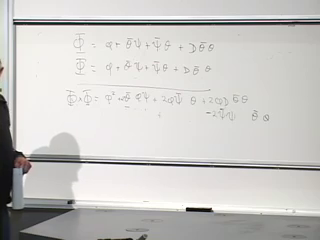
\includegraphics[width=0.82\textwidth]{lecture_07_figure_05.png}
\lectureframe{01:07:57.844}
\caption{Tích siêu trường theo từng thành phần và việc thu gom các hạng \(\bar\theta\theta\) của nó.}
\end{figure}

Hai hạng \(\phi D\) và \(D\phi\) cộng lại vì cả hai trường đều chẵn. Hai hạng chéo fermion cũng cộng lại sau khi mỗi hạng được sắp xếp lại, nhưng dấu chung của chúng là âm:
\begin{equation}
(\bar\theta\psi)(\bar\psi\theta)
+(\bar\psi\theta)(\bar\theta\psi)
=-2\bar\psi\psi\,\bar\theta\theta.
\end{equation}
Tích phân bình phương ấy theo các tọa độ lẻ cho
\begin{equation}
\int d\theta\,d\bar\theta\;\Phi^2
=2\phi D-2\bar\psi\psi.
\end{equation}
Hạng này là siêu đối xứng do được xây dựng như vậy, nhưng nó vẫn chưa phải là một Lagrangian động năng. Nó không chứa đạo hàm theo thời gian.

Sau đó trên bảng đề xuất \(\Phi^3\), \(\Phi^4\) và \(\Phi^n\) làm bài tập. Có một quy tắc gọn. Với mọi hàm thường \(W\),
\begin{equation}
\left.W(\Phi)\right|_{\bar\theta\theta}
=W'(\phi)D-W''(\phi)\bar\psi\psi.
\label{eq:l7-function-top-component}
\end{equation}
Với \(W(\phi)=\phi^2\), ta khôi phục lại phương trình~\eqref{eq:l7-superfield-square}; với \(W(\phi)=\phi^n\), ta được
\begin{equation}
\left.\Phi^n\right|_{\bar\theta\theta}
=n\phi^{n-1}D-n(n-1)\phi^{n-2}\bar\psi\psi.
\end{equation}
\editorialnote{Bài giảng giao lũy thừa bậc \(n\) làm bài tập và nêu các loại hạng tử được mong đợi. Phương trình~\eqref{eq:l7-function-top-component} cho quy tắc hoàn chỉnh trong quy ước thứ tự cố định.}

Tới đây giảng viên hỏi liệu cả phòng có kiệt sức chưa. Khán giả đáp là chưa; ông trả lời rằng người kiệt sức là ông. Trao đổi ấy không chỉ để gây cười. Lũy thừa của siêu trường thì dễ vì khai triển dừng lại, nhưng đạo hàm và ràng buộc mới là chỗ việc theo dõi dấu trở nên thực sự đòi hỏi.

\section{Những đạo hàm nào tương thích với siêu đối xứng?}

Có một chỗ cần sửa trước khi theo dõi lập luận tiếp theo trên bảng. Đạo hàm thời gian thông thường là vô hại:
\begin{equation}
[\partial_t,q]=[\partial_t,\bar q]=0.
\end{equation}
Do đó \(\partial_t\Phi\) biến đổi như một siêu trường mỗi khi \(\Phi\) biến đổi như vậy. Những đối tượng tinh tế là các đạo hàm lẻ trần \(\partial_\theta\Phi\) và \(\partial_{\bar\theta}\Phi\), vì chúng không phản giao hoán với cả hai siêu điện tích. Ta cần các đạo hàm lẻ đã hiệu chỉnh cho các ràng buộc và cho các phép xây dựng theo thành phần hiển nhiên siêu đối xứng.
\editorialnote{Phát biểu bằng lời rằng phép vi phân theo thời gian không cho ra một siêu trường khác là không đúng trong quy ước được dùng ở đây. Vì \(\partial_t\) giao hoán với cả hai siêu điện tích nên nó là hiệp biến. Việc xây dựng tiếp theo các đạo hàm lẻ đã hiệu chỉnh vẫn là cần thiết và mới là điểm toán học thực sự của bài giảng.}

\subsection{Phép tương tự ``trường ma thuật''}

Bài giảng nêu động cơ cho tiêu chuẩn này bằng các phép quay thông thường. Cho \(f(x,y)\) thỏa mãn
\begin{equation}
\partial_y f=0.
\label{eq:l7-magic-constraint}
\end{equation}
Hãy gọi một hàm như vậy là ``trường ma thuật.'' Nó phụ thuộc vào \(x\) nhưng không phụ thuộc vào \(y\). Lớp các trường ma thuật có được bảo toàn dưới phép quay không? Với
\begin{equation}
L_z=-i\left(x\partial_y-y\partial_x\right),
\end{equation}
ta tìm được
\begin{equation}
[\partial_y,L_z]=i\partial_x\neq0.
\end{equation}
Vì vậy \(L_z f\) nói chung sẽ nhận thêm phụ thuộc vào \(y\) ngay cả khi ban đầu \(f\) thỏa phương trình~\eqref{eq:l7-magic-constraint}. Ràng buộc ấy không bất biến quay.

Bài học tổng quát thì đơn giản. Nếu một trường thỏa \(C\Phi=0\) và một đối xứng được sinh bởi \(G\), thì trường đã biến đổi vẫn còn bị ràng buộc khi giao hoán tử phân bậc của \(C\) và \(G\) triệt tiêu. Đối với hai toán tử lẻ, giao hoán tử phân bậc là một phản giao hoán tử.

\begin{classroomqa}
\audiencequestion{Khi nào một ràng buộc đặt lên một trường là tương thích với một đối xứng? \lecturetimestamp{01:17:56}}
\lecturerresponse{Khi toán tử ràng buộc giao hoán phân bậc với các bộ sinh đối xứng. Khi đó \(C(G\Phi)\) có thể được đưa qua \(G\) và rút về \(G(C\Phi)=0\). Ví dụ về phép quay thất bại vì \(\partial_y\) không giao hoán với bộ sinh quay.}
\end{classroomqa}

\subsection{Các đạo hàm lẻ hiệp biến}

Với các siêu điện tích được cố định bởi phương trình~\eqref{eq:l7-differential-supercharges}, hãy định nghĩa
\begin{equation}
\mathcal D=\partial_\theta-i\bar\theta\partial_t,
\qquad
\bar{\mathcal D}=\partial_{\bar\theta}-i\theta\partial_t.
\label{eq:l7-covariant-derivatives}
\end{equation}
Thay đổi duy nhất là dấu của hạng đạo hàm theo thời gian. Tính trực tiếp cho
\begin{align}
\{\mathcal D,q\}
&=\{\mathcal D,\bar q\}
=\{\bar{\mathcal D},q\}
=\{\bar{\mathcal D},\bar q\}=0,\\
\{\mathcal D,\bar{\mathcal D}\}&=-2i\partial_t.
\label{eq:l7-covariant-algebra}
\end{align}
Hai hạng chéo có thể khác không triệt tiêu lẫn nhau. Đây là phép tương tự lẻ của một đạo hàm hiệp biến: nó lấy đạo hàm mà vẫn bảo toàn luật biến đổi.

Bài giảng dùng \(D\) vừa cho thành phần phụ trợ vừa cho đạo hàm này. Ta dành \(D(t)\) cho thành phần và dùng dạng thư pháp \(\mathcal D\) cho toán tử.

\section{Ràng buộc chiral}

Giờ đây ta có thể áp đặt một ràng buộc không tầm thường vẫn được bảo toàn bởi siêu đối xứng:
\begin{equation}
\bar{\mathcal D}\Phi=0.
\label{eq:l7-chiral-constraint}
\end{equation}
Một trường như vậy được gọi là chiral. Nếu nó là chiral trước một phép biến đổi siêu đối xứng, thì
\begin{equation}
\bar{\mathcal D}(q\Phi)
=-q(\bar{\mathcal D}\Phi)=0,
\qquad
\bar{\mathcal D}(\bar q\Phi)
=-\bar q(\bar{\mathcal D}\Phi)=0.
\end{equation}
Vì thế toàn bộ siêu trường đã biến đổi vẫn nằm trong lớp bị ràng buộc ấy. Khác với điều kiện trường ma thuật, tính chiral là tương thích với đối xứng.

Để giải ràng buộc, hãy định nghĩa một tọa độ thời gian dịch chuyển
\begin{equation}
\tau=t+i\bar\theta\theta.
\label{eq:l7-chiral-time}
\end{equation}
Vì ta dùng đạo hàm trái,
\begin{equation}
\partial_{\bar\theta}\tau=i\theta,
\end{equation}
và do đó
\begin{equation}
\bar{\mathcal D}F(\tau,\theta)
=\left(\partial_{\bar\theta}-i\theta\partial_t\right)F(\tau,\theta)
=i\theta\partial_\tau F-i\theta\partial_\tau F=0.
\end{equation}
Vì vậy siêu trường chiral cục bộ tổng quát chỉ phụ thuộc vào \(\bar\theta\) thông qua \(\tau\):
\begin{equation}
\Phi_{\mathrm{ch}}(\tau,\theta)
=\phi(\tau)+\bar\psi(\tau)\theta.
\label{eq:l7-chiral-field-tau}
\end{equation}

\begin{classroomqa}
\audiencequestion{Sự phụ thuộc vào \(\tau\) và \(\theta\) có phải là dạng duy nhất thỏa ràng buộc chiral không? \lecturetimestamp{01:32:35}}
\lecturerresponse{Xét cục bộ thì có. Phương trình vi phân \(\bar{\mathcal D}\Phi=0\) nói chính xác rằng sự phụ thuộc độc lập vào \(\bar\theta\) có thể được hấp thụ vào tọa độ dịch chuyển \(\tau=t+i\bar\theta\theta\). Khai triển hữu hạn còn lại là một hàm của \(\tau\) cộng với một hạng tỉ lệ với \(\theta\).}
\end{classroomqa}

Khai triển lại theo tọa độ thời gian ban đầu,
\begin{align}
\phi(\tau)
&=\phi(t)+i\bar\theta\theta\dot\phi(t),\\
\bar\psi(\tau)\theta
&=\bar\psi(t)\theta,
\end{align}
vì hiệu chỉnh ở dòng thứ hai chứa \(\theta^2\). Do đó
\begin{equation}
\Phi_{\mathrm{ch}}(t,\theta,\bar\theta)
=\phi(t)+\bar\psi(t)\theta
+i\bar\theta\theta\dot\phi(t).
\label{eq:l7-chiral-field-components}
\end{equation}

\begin{classroomqa}
\audiencequestion{Khai triển Taylor của \(\phi(t+i\bar\theta\theta)\) có nên chứa một hạng bậc hai không? \lecturetimestamp{01:33:51}}
\lecturerresponse{Không. Hiệu chỉnh đầu tiên là \(i\bar\theta\theta\dot\phi\), và mọi hiệu chỉnh bậc cao hơn đều chứa \((\bar\theta\theta)^2=0\). Khán giả nhận ra điều này ngay lập tức; tính lũy linh đã cung cấp hai hạng đầu và chấm dứt chuỗi.}
\end{classroomqa}

Đó là sự gọn nhẹ của tính chiral. Siêu trường không bị ràng buộc trong phương trình~\eqref{eq:l7-superfield} có hai vị trí thành phần bosonic và hai vị trí thành phần fermionic. Điều kiện chiral loại bỏ vị trí phụ trợ độc lập trong ví dụ một chiều tối thiểu này và gắn thành phần trên cùng với \(\dot\phi\).

\section{Phép tính dừng lại đúng lúc}

Bước tiếp theo tự nhiên là kết hợp trường chiral với trường liên hợp của nó và lấy tích phân trên siêu không gian. Việc khai triển liên hợp được bắt đầu, và một người nghe hỏi liệu thứ tự \(\theta\bar\theta\) có phải đảo ngược dưới phép liên hợp hay không. Đến lúc ấy các dấu không còn có vẻ đáng tin nữa. Thay vì đoán bừa, phép tính dừng lại.

\begin{classroomqa}
\audiencequestion{Liệu ta có thể nghe kết luận chính ngay cả khi phép nhân với trường liên hợp được để lại sau không? \lecturetimestamp{01:37:30}}
\lecturerresponse{Có. Nếu các dấu và các phép liên hợp được xử lý nhất quán, một biểu thức trong siêu không gian xây từ một trường chiral và trường liên hợp của nó sẽ cho ra các hạng động năng bosonic và fermionic thông thường như mong muốn. Kết quả quan trọng đối với bài giảng này là nguyên lý xây dựng, chứ không phải một dòng cuối thiếu tin cậy được chép ra từ một phép tính khi đã mệt.}
\end{classroomqa}

Điểm dừng ấy nên được giữ rõ. Hình thức luận này không khoan nhượng: chỉ cần đặt sai một thừa số lẻ là đổi dấu, và cùng một quy ước phải được duy trì qua phép liên hợp, phép vi phân, phép nhân và phép tích phân. Phản ứng đúng khi làm mất mạch đó là sửa lại nó trước khi đi tiếp. Trong một quy ước chuẩn, tác dụng động năng quen thuộc được xây từ một tích liên hợp, nhưng phép rút gọn chi tiết theo thành phần của nó thuộc về phép tính sạch sẽ kế tiếp, chứ không phải việc phục dựng một dòng dang dở trên bảng.

\section{Vì sao đối xứng mới là điểm mấu chốt}

Một Lagrangian siêu đối xứng không chỉ đặt một boson và một fermion cạnh nhau. Nó ràng buộc khối lượng và tương tác của chúng sao cho chúng tạo thành một biểu diễn của siêu đại số. Trong một chân không siêu đối xứng chính xác, các thành viên của một siêu bội có khối lượng bằng nhau. Các đóng góp vòng của chúng có tương quan, và các hiệu ứng tử ngoại bosonic và fermionic triệt tiêu đúng trong những tổ hợp mà đối xứng áp đặt.

Đó là lý do bộ máy xây dựng này quan trọng. Ta có thể liệt kê các đỉnh Feynman và kiểm tra sự triệt tiêu sơ đồ này qua sơ đồ khác, nhưng khi ấy các sự triệt tiêu sẽ có vẻ ngẫu nhiên. Siêu đối xứng giải thích chúng theo đúng cách mà đối xứng Lorentz giải thích vì sao các biên độ tán xạ biến đổi nhất quán trong mọi hệ quy chiếu quán tính.

\editorialnote{Siêu đối xứng chính xác không hàm ý rằng mọi hiệu chỉnh tự năng lượng riêng lẻ đều triệt tiêu. Nó liên hệ các sự tái chuẩn hóa và loại bỏ những độ nhạy tử ngoại nhất định; các mệnh đề không tái chuẩn hóa phụ thuộc vào đại lượng xét đến, số chiều và số lượng siêu đối xứng. Phát biểu khái quát của bài giảng về sự triệt tiêu được giữ lại dưới dạng có điều kiện này.}

\begin{classroomqa}
\audiencequestion{Từ ``chiral'' được đánh vần thế nào? \lecturetimestamp{01:39:48}}
\lecturerresponse{C-H-I-R-A-L. Từ này dùng để chỉ ràng buộc \(\bar{\mathcal D}\Phi=0\); nó không phải là tính thuận tay hình học thông thường của một vật trong không gian ba chiều, mặc dù thuật ngữ này bắt nguồn từ cấu trúc tay trái và tay phải của các spinor tương đối tính.}
\end{classroomqa}

\begin{classroomqa}
\audiencequestion{Liệu có thể bỏ qua Lagrangian và đi thẳng tới các quy tắc Feynman siêu đối xứng không? \lecturetimestamp{01:40:00}}
\lecturerresponse{Dĩ nhiên ta có thể phát biểu các quy tắc đó, nhưng khi ấy các quan hệ giữa những hằng số ghép và các sự triệt tiêu do chúng tạo ra sẽ trông như những sự trùng hợp không có lời giải thích. Nội dung sâu hơn là đối xứng không-thời gian được tổng quát hóa. Lagrangian, hoặc một hình thức bất biến tương đương, làm lộ rõ nguyên nhân đó và sinh ra các quy tắc một cách có hệ thống.}
\end{classroomqa}

Giả sử mọi bậc của lý thuyết nhiễu loạn đều tình cờ cho ra các biên độ bất biến Lorentz mặc dù chưa hề nhắc đến các phép biến đổi Lorentz nào. Sau đủ nhiều phép tính, ta sẽ đòi hỏi một lời giải thích. Câu trả lời sẽ là đối xứng không-thời gian tổ chức mọi bậc ấy cùng một lúc. Vai trò của siêu không gian là tương tự: các dịch chuyển theo \(\theta,\bar\theta\) trộn các thành phần boson và fermion, và đại số của chúng khép kín thành các phép tịnh tiến trong không-thời gian.

\begin{classroomqa}
\audiencequestion{Có nên khai triển cả các tọa độ không gian thông thường thành một chuỗi lũy thừa hữu hạn, như đối với các tọa độ Grassmann, không? \lecturetimestamp{01:44:55}}
\lecturerresponse{Không. Một chuỗi lũy thừa theo một tọa độ thông thường không kết thúc và thường không phải là cách phân tích tự nhiên. Phép biến đổi Fourier hữu ích hơn vì nó phân giải một trường thành các sóng và các xung lượng. Việc khai triển theo \(\theta\) là đặc biệt chính vì tính lũy linh làm cho nó hữu hạn.}
\end{classroomqa}

\begin{classroomqa}
\audiencequestion{Nếu một hạt mới xuất hiện tại LHC, làm sao ta có thể biết đó là một siêu đối tác chứ không chỉ đơn thuần là một hạt chưa biết? \lecturetimestamp{01:45:42}}
\lecturerresponse{Siêu đối xứng dự đoán các số lượng tử và các tương tác có tương quan với nhau, chứ không chỉ một trạng thái bổ sung đơn lẻ. Spin chênh nhau một nửa, các điện tích chuẩn có liên hệ với nhau, và nhiều hằng số ghép bậc ba và bậc bốn được chi phối bởi ít tham số độc lập hơn so với trong một lý thuyết tổng quát. Các tiết diện, các tỉ phần rẽ nhánh và phần còn lại của phổ sẽ phải thỏa mãn những quan hệ đó.}
\end{classroomqa}

Một cộng hưởng lạ tự nó sẽ không chứng minh được siêu đối xứng. Thứ có thể làm được điều đó là một mạng lưới các quan hệ về hằng số ghép và phổ. Đó là đối ứng thực nghiệm của phép xây dựng siêu không gian: các tương tác thành phần có vẻ độc lập đều xuất phát từ một đối tượng bất biến.

\begin{classroomqa}
\audiencequestion{Các hạt đã quan sát được và các siêu đối tác giả thuyết của chúng không có cùng khối lượng. Điều đó làm thay đổi lý thuyết như thế nào? \lecturetimestamp{01:47:01}}
\lecturerresponse{Nó làm lý thuyết thay đổi rất nhiều. Siêu đối xứng phải bị phá vỡ, thường thông qua sự phá vỡ tự phát được truyền sang ngành quan sát được. Sự phá vỡ ấy làm tách các khối lượng trong đa bội, đồng thời vẫn giữ lại đủ cấu trúc để khống chế các tương tác và, nếu thang năng lượng đủ thấp, các hiệu chỉnh tử ngoại. Việc xây dựng chi tiết cơ chế đó tự nó đã là một lý thuyết đáng kể, đặc biệt khi đưa hấp dẫn vào.}
\end{classroomqa}

\section{Nguyên lý đơn giản, phép tính khó}

Nhận định kết thúc này thẳng thắn một cách khác thường. Ý tưởng ban đầu nghe có vẻ đơn giản: boson và fermion liên hệ với nhau bởi một đối xứng. Thế nhưng việc triển khai nhanh chóng trở thành một công việc của chỉ số, các phép liên hợp, thứ tự Grassmann và dấu. Ngay cả sau khi đã xây dựng được đối xứng ấy, vật lý hạt hiện thực vẫn đòi hỏi phải phá vỡ nó; ghép nó với hấp dẫn sẽ dẫn tới siêu hấp dẫn và thêm một tầng cấu trúc nữa.

Sự khó khăn này không phải là bằng chứng cho thấy ý tưởng đó trống rỗng. Tự nhiên không có nghĩa vụ phải khiến một nguyên lý đơn giản trở nên dễ tính toán. Các chuyên gia học chủ đề này bằng cách lặp đi lặp lại các chi tiết cho đến khi các quy tắc về dấu trở thành phản xạ tự nhiên. Sự bực bội bắt nguồn từ khoảng cách giữa đại số cô đọng
\begin{equation}
\{Q,Q^\dagger\}=2H
\end{equation}
và lượng công cụ cần thiết để hiện thực hóa nó trong một lý thuyết có tương tác.

\begin{classroomqa}
\audiencequestion{Liệu cuối cùng một tầng trừu tượng hóa nữa có đơn giản hóa hình thức luận hay không, hay sự phức tạp cứ tiếp tục tích lũy? \lecturetimestamp{01:49:33}}
\lecturerresponse{Không có sự đơn giản hóa tổng quát nào loại bỏ được phần việc chi tiết. Các quy tắc nền tảng có thể ngắn gọn, nhưng việc dùng chúng một cách đáng tin cậy đòi hỏi phải liên tục kiểm soát các quy ước. Đó là lý do vì sao một trình bày đầy đủ thường chiếm trọn một học phần kỹ thuật, chứ không chỉ là một phần nhỏ của một học phần vật lý hạt tổng quát.}
\end{classroomqa}

\begin{classroomqa}
\audiencequestion{Các phép biến đổi đó có cho ta biết fermion và boson thực sự là gì, hoặc vì sao hành vi thông thường của chúng khác nhau không? \lecturetimestamp{01:51:42}}
\lecturerresponse{Chúng cho ta biết rằng cả hai là các thành phần của một siêu trường và được ánh xạ thành nhau dưới tác dụng của các siêu tích. Tác dụng bằng \(Q\) sẽ ánh xạ một thành phần boson thành một thành phần fermion, còn phép biến đổi kế tiếp tạo ra các đạo hàm và các thành phần phụ trợ. Điều này tương tự với một phép quay trộn các thành phần vectơ, nhưng không thể diễn dịch nó thành một bức tranh cũng trực tiếp theo nghĩa đen như vậy: ngôn ngữ thích hợp chính là bản thân hình học Grassmann.}
\end{classroomqa}

Câu trả lời đó đưa ta trở lại ý tưởng trung tâm. Một phép biến đổi siêu đối xứng là một dịch chuyển nhỏ trong siêu không gian. Nó trộn \(\phi,\psi,\bar\psi,D\) giống như một phép quay thông thường trộn các thành phần, và làm như vậy đồng thời khép kín thành một phép tịnh tiến theo thời gian. Bức tranh này mang tính trừu tượng, nhưng không hề tùy tiện: mọi hạng trong siêu trường, mọi dấu trong các đạo hàm hiệp biến và mọi quan hệ giữa các tương tác thành phần đều tồn tại để hiện thực hóa đại số đó.

\section{Những gì chúng ta đã xây dựng}

Chúng ta bắt đầu với Hamiltonian của dao động tử ghép cặp và khôi phục hai mô tả Lagrangian khác nhau của nó. Boson tuân theo một phương trình dao động tử bậc hai; fermion đòi hỏi một tác dụng Grassmann bậc nhất và một cặp thành phần lẻ phức. Các siêu tích hoán đổi hai mode, tự bình phương từng cái đều bằng không, phản giao hoán với nhau để cho Hamiltonian, và giao hoán với Hamiltonian.

Việc biểu diễn các siêu tích ấy như các toán tử vi phân đã dẫn tới siêu không gian. Một khai triển siêu trường hữu hạn đã tập hợp các thành phần boson, fermion và phụ trợ; phép lấy tích phân Berezin đã chọn ra thành phần cao nhất của một siêu Lagrangian; và phép nhân đã sinh ra các ứng viên tương tác bất biến. Yêu cầu về phép vi phân lẻ tương thích với đối xứng sau đó dẫn tới \(\mathcal D,\bar{\mathcal D}\), ràng buộc chiral và tọa độ dịch chuyển \(\tau=t+i\bar\theta\theta\).

Phép tính tích liên hợp còn dang dở là một phần của bài học chứ không phải một khuyết điểm cần che giấu. Siêu đối xứng bắt đầu từ một đòi hỏi vật lý đơn giản, nhưng phép tính của nó nhạy với mọi lựa chọn thứ tự. Một khi đã kiểm soát được những lựa chọn đó, thành quả là rất lớn: khối lượng và các hằng số ghép được tổ chức bởi đối xứng, các hiệu chỉnh lượng tử thỏa mãn những quan hệ không phải ngẫu nhiên, và boson cùng fermion trở thành các thành phần của một đối tượng hình học duy nhất.